\documentclass[a4paper,11pt]{article}

\usepackage[utf8]{inputenc}    % Pour que LaTeX comprenne les accents.
\usepackage{times}             % Police de caractères
\usepackage[english]{babel}     % Traitement du texte adapté aux règles typographiques
                               % de la langue donnée en option (e.g., pour l'espacement
                               % après les ponctuations
\usepackage[T1]{fontenc}
\usepackage{amsmath, amsthm, amssymb} 
\usepackage{dsfont}  % pour les indicatrices 
\usepackage{graphicx} 
\usepackage{textcomp}                               
\sloppy              % Ne pas faire déborder les lignes dans la marge


\newtheorem{lemma}{Lemma}
\newtheorem{cons}{Corollary}
\newtheorem{theo}{Theorem}

\theoremstyle{definition}
\newtheorem{definition}{Definition}
\newtheorem{process}{Process}

\theoremstyle{remark}
\newtheorem{remark}{Remark}

\title{Throwing needles on a coloured plane.}

\begin{document}
\maketitle

\begin{abstract}  In this paper, we study $n$-colourings of plane 
that maximize the probability that when throwing a needle in the plane the two 
endpoints of the needle have different colours. Our major result establish a 
correlation between $n$-colouring of plane and finite unit-distance graphs. 
It provides some bounds for the optimal probability.\end{abstract}

\section{Introduction}
This idea of throwing a needle on a coloured floor was somehow motivated by 
the announcement of cell phones chargers that are simple surfaces where a cell 
phone can be put to start charging. Imagine that the endpoints 
represent two electrodes on our cell phone, and that the colours represent 
different electric potentials on the conductive plane~: we would try to make 
the colouring optimal so that the cell phone can be charged with a big enough 
probability. Of course, actual implementations of that technology are not so 
simple.

The problem we are interested in is the following : if $c$ is a 
\emph{valid} colouring the plane with $n$ colours, in a  way that will be 
defined further, define $p(c)$ as the probability that when throwing a needle 
on $c$, both endpoints have the same colour. What is the minimal $p(c)$ with a 
fixed number of colours $n$, and for what colourings is it obtained ?

This can be seen as a probabilistic version of the well known 
\emph{Hadwiger-Nelson problem}. This problem asks for the chromatic number 
of the euclidian plane, where unit-distance points are connected. Some 
relations with our problem will be presented in paragraph~\ref{hn}. One can 
first remark that knowing that the answer to the Hadwiger-Nelson problem is at 
most $7$, with a $7$-colouring of the plane such that two unit distance points 
always have different colours, the maximum probability we are looking for is 
$1$ if $n \geq 7$.

In section~\ref{def} we define the process more precisely. In particular, we 
need to make some assumption on the colouring for the probability to make 
sense. Our main result, establishing links between finite graphs and our 
probability, is presented in section~\ref{equiv}. We then show some 
consequences, and try to generalise this idea in higher dimensions in
section~\ref{appli}. Finally, we study in section~\ref{fini} the problem of 
throwing a needle on a finite table.

\section{Definitions}
\label{def}
First, we call \emph{colouring} a function $c$ from the euclidian plane to the 
set of colours, represented by the integers $ [| 1 ; n |]$. For the probability 
to be well defined, we will 
first require that every set $U_i = c^{-1}(i)$ for $i \in [| 1 ; n |]$ be 
Lebesgue-measurable - equivalently, that the function $c$ itself be 
Lebesgue-measurable. Since it's impossible to ``throw a needle uniformly on the 
whole plane'', we also choose to make the following assumption : 
the colouring has to be \textit{periodic} - that is, there are some free vectors 
$u$ and $v$ such that translations along these vectors leave the colouring 
unchanged.

A colouring is said to be \emph{valid} if it is Lebesgue-measurable and 
periodic. Thereafter, we 
will always assume that the colouring is valid. We will denote $\mathbf{P}$ the 
parallelogram defined by the two vectors of periodicity. Using periodicity, 
we can then throw needles on this parallelogram only, so 
that probabilities actually make sense.
\begin{remark}
Note that there are several couples of vectors $(u,v)$ forming an appropriate 
basis for the colouring. Nonetheless, it's clear that probabilities do not 
depend on that choice. 
\end{remark}

The notion of a \emph{unit distance graph} will also be useful~:
\begin{definition}

A finite graph $(V,E) $ is said to be \emph{unit distance} if it has a 
representation in the plane in which all edges have length $1$.
\end{definition}

We now define formally the needle-throwing process we use to study probabilities. 
In this definition, and throughout the whole paper, when no further precision 
is given the words ``uniform'' and ``uniformly'' refer to the Lebesgue measure -
except when we chose in a finite set, where it has its usual meaning.
\begin{process}
Consider the following random variables :
\begin{itemize}
  \item let $A$ (the lowest end of the needle) be a point chosen uniformly 
  in $\mathbf{P}$ ;
  \item let $\theta$ be an independent angle chosen uniformly in $[0;\pi[$ ;
  \item let $A$ (the highest end of the needle) be $A + e^{i \theta}$.
\end{itemize}
\end{process}

Note that $B$ may fall outside of $\mathbf{P}$. In that case, $c(B)$ is 
defined using the periodicity of the colouring.
Our goal is to evaluate and minimize the probability that both ends have the 
same color.

We consider the following, second process that will be very useful in our 
proofs. The idea is to throw a unit distance graph on the 
plane, and then to choose a needle on that graph~:
\begin{process}
Given a unit distance graph $(G,V)$, implicitly represented in the plane in 
a unit distance way, label the edges with numbers from 
$1$ to $m$. Choose~: 
\begin{itemize}
\item one point $A_0$ uniformly on the initial parallelogram $\mathbf{P}$ for 
the origin of the graph ;
\item an independent angle $\theta$ uniformly in $[0;2\pi[$, to rotate the graph ;
\item an independent index $i$ in $[| 1;m|]$.
\end{itemize}
Then, rotate the graph by the angle $\theta$, translate it so that the origin 
falls on  $A_0$, and take the needle $(A',B')$ corresponding to the $i^{th}$ 
edge of the obtained graph.
\end{process}

\section{Process equivalence}
\label{equiv}
\begin{lemma}\label{huitre}
Let $(A,B)$ be the needle obtained by the first process, and
$(A',B')$ the one obtained by the second process. Let $c_1$ and $c_2$ denote 
two colors, and $c$ a valid colouring. Then, we 
have~:\\
 $$\mathbb{P}(c(A) = c_1 , c(B) = c_2) = \mathbb{P}(c(A') = c_1, c(B') = c_2) $$ \\
 In particular, the probability doesn't depend on the graph 
 chosen. For a graph with only two vertices, we exactly get the initial process.
\end{lemma}

\begin{proof}
Conventions : 
\begin{itemize}
\item we take a graph $G=(V,E)$, and $m = |E|$, the number of edges.

\item as usual, $\mathbf{P}$ is the parallelogram obtained by the periodicity 
of the colouring.

\item $\mathcal{A}(\mathbf{P})$ is the area of the parallelogram

\item $i \in [|1;m|]$ is the index of one of the edges of $G$.

\item $\theta_i$ denotes the angle made by a horizontal line and the $i^{th}$ 
edge of the graph. The 
complex coordinates of the vertices of the $i^{th}$ edges before 
rotation/translation are named $z_i $ and $z_i + e^{i.\theta_i}$.

\end{itemize}

We prove our lemma by the following series of equalities :

\begin{eqnarray*}
& & \mathbb{P}(c(A') = c_1, c(B') = c_2) \\
  &=& \frac{1}{m}\sum_{i=1}^{m} \mathbb{P}(c(A') = c_1, c(B') = c_2 | i)  \\
  &=& \frac{1}{m}\sum_{i=1}^{m}  \frac{1}{2\pi}\int_{\theta =0} ^{2\pi} \frac{1}{\mathcal{A}(\mathbf{P})}\int\int_{A_0 \in \mathbf{P}} \mathbb{P}(c(A') = c_1, c(B') = c_2 | i, \theta, A_0) d\theta dx dy \\  
  &=& \frac{1}{m 2\pi \mathcal{A}(\mathbf {P})}\sum_{i=1}^{m}\int_{\theta =0} ^{2\pi} \int\int_{A_0 \in \mathbf{P}} \mathds{1}(c(A_0 + z_i e^{i\theta}) = c_1, c(A_0 +z_i e^{i\theta} + e^{i (\theta + \theta_i)}) = c_2) d\theta dx dy \\  
    &=& \frac{1}{m 2\pi \mathcal{A}(\mathbf{P})}\sum_{i=1}^{m} \int_{\theta =0} ^{2\pi} \int\int_{A_0 \in \mathbf{P}} \mathds{1}(c(A_0) = c_1, c(A_0 + e^{i (\theta + \theta_i)}) = c_2 ) d\theta dx dy \hspace{1 cm} (*)\\ 
    &=& \frac{1}{m 2\pi \mathcal{A}(\mathbf{P})}\sum_{i=1}^{m} \int_{\theta =0} ^{2\pi} \int\int_{A_0 \in \mathbf{P}} \mathds{1}(c(A_0) = c_1, c(A_0 + e^{i \theta}) = c_2 ) d\theta dx dy \\ 
    &=& \frac{1}{2\pi \mathcal{A}(\mathbf{P})}\int_{\theta =0} ^{2\pi} \int\int_{A_0 \in \mathbf{P}} \mathds{1}(c(A_0) = c_1, c(A_0 + e^{i \theta}) = c_2 ) d\theta dx dy \\ 
\end{eqnarray*}
Which gives exactly the same probability as the first process (except that the 
angle is taken in $[0;2\pi[$ here, instead of $[0;\pi[$, but it doesn't make 
any difference when looking only at the colors).

Equality $(*)$ is justified by the periodicity of our colouring.
\end{proof}

\begin{cons} \label{ineg}
$$ \max_{g \in G} c_n(g) \leq \min_{c \in C_n} p(c) $$
where \begin{itemize} 
  \item $G$ is the set of finite unit-distance graphs 
  \item $C_n$ is the set of valid $n$-colourings.
  \item $c_n(g)$ is the minimal number of edges having the same colours of both 
ends when colouring the graph $g$ with $n$ colours, divided by the 
number of edges in $g$
(for example, $\frac 1 {3}$ for an equilateral triangle with $n=2$.)
  \item $p(c)$ is the probability of getting the same colour on both ends, when 
throwing a needle on the colouring $c$.
\end{itemize}

\end{cons}

\begin{proof}
Consider a graph $g$ coloured with $n$ colours. When one chooses a needle
randomly on this graph the probability that both ends have the same
colours is clearly greater than $c_n(g)$. Applying lemma \ref{huitre} with $g$, 
it follows from the description of the second process that the probability 
$p(c)$ for any colouring $c$ is greater than $c_n(g)$.
\end{proof}
We still don't know wether or not this is actually an equality. It is for 
$n=2$, as will be shown thereafter.

\section{Applications} \label{appli}
\subsection{2 colours}


With two colors, we consider a triangle as our graph. 
As there is always at least two vertices with the same color, it's clear that 
the probability that $c_2(g) = \frac{1}{3}$. Thanks to Corollary~\ref{ineg}, 
we know that $p(c) \geq \frac13$ for any valid $c$.

This bound is optimal. Indeed, consider the colouring in figure~\ref{color}, 
constructed with parallel strips of width 
$l = \frac {\sqrt3}{2}$, with the upper side opened and the lower side closed. 
It is clearly a valid colouring.  
%IMAGE DU COLORIAGE + preuve optimalité
\begin{figure}[h]
\center
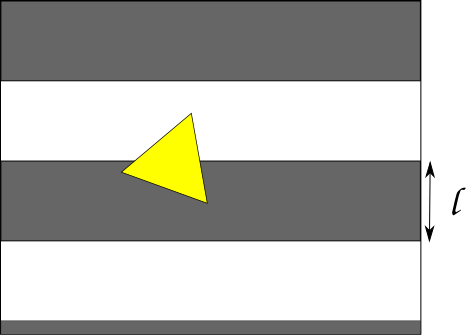
\includegraphics[scale=0.5]{path6509.png}
\caption{\label{couleur} The parallel stripes $2$-colouring}
\end{figure}

For this colouring, the probability of getting the same colour using the first 
process is $\frac13$. This fact can be shown by direct computation, or one can 
more simply remark that no unit-lengthed equilateral triangle can have its 
three vertices with the same colors. Applying Lemma~\ref{huitre}, we conclude 
that this colouring achieves a probability of $\frac{1}{3}$ indeed.
%CLASSE DE SOLUTIONS?

\subsection{3 colours}
 With three colors, we use the Moser spindle of Figure~\ref{color} - that 
 has at least one of its $11$ edges with both ends of the same colour.
 We similarly get that for $n=3$, the probability that both endpoints have the 
 same colour is at least 
 $\frac{1}{11}$ for any valid colouring. 

\begin{figure}[h]
\center
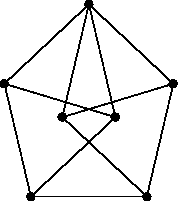
\includegraphics[scale=0.4]{T.png}
\caption{\label{color} The Moser spindle}
\end{figure}

We don't know if the previous bound is optimal. We believe that Figure~\ref{trois} 
can give a rather good $3$-colouring of the plane, for some well chosen length 
of the edge of the hexagons. Rough simulations have shown that this gave us a 
$p$ of about $0.12$ for an edge of length about $0.61$. 
Still, we did not compute the exact optimum in that case because this 
estimation is still far away from $\frac{1}{11}$.

\begin{figure}[h]
\center
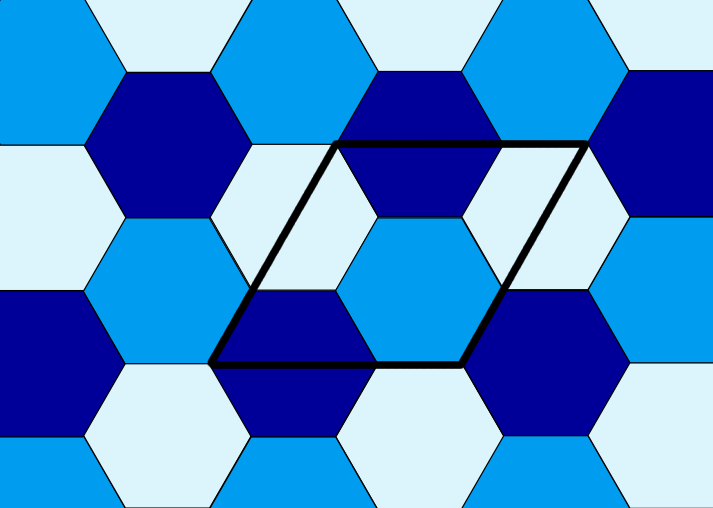
\includegraphics[scale=0.5]{trois.png}
\caption{\label{trois} A hexagonal $3$-colouring and its parallelogram of periodicity}
\end{figure}
  %Mettre les exemples de coloriages, avec les probas obtenues.

\subsection{Other extensions}
\label{dim}

The previous considerations can be extended to dimension $d \geq 3$, however, 
it becomes more complicated to write down. We have to consider a basis of 
vector leaving our colouring unchanged, and still denote by $\mathbf{P}$ the 
parallelepiped induced by these vectors.

The first process for choosing a needle now consist in~: 
\begin{itemize}
	\item choosing one point uniformly in the parallelepiped $ \mathbf{P} $ as 
	one point of the needle~;
	\item choosing independently one point uniformly on the unit sphere 
	$S^{d-1}$, uniformly to give the relative position of the second point.
\end{itemize}

Sending a unit-length graph on the $d$-dimensional space becomes somehow more 
complicated. We have to choose one initial point in $ \mathbf{P} $, and an independent 
rotation of our graph uniformly among vectorial rotations~; this can be achieved 
by using the Haar measure of $SO(d)$ uniformly. The second process now consists 
in~: rotating the graph thanks to the matrix of $SO(d)$ chosen, translating it 
to the point of $\mathbf{P}$ chosen, and chosing one of the 
edges independently as your needle.

One can verify that the proof of Lemma~\ref{huitre} adapts to that definitions. 
It means that previous results still hold - namely, the probability that both 
ends fall on the same colour remains the same for the two processes. Crucial 
points are the invariance of the Haar measure under matrix product, and the 
fact that the image measure of said Haar measure by the application 
$M\mapsto Mv$, where $v$ is a given unit vector, is the uniform Lebesgue 
measure of $S^{d-1}$.

Thus, to find lower bonds on our probability, the same techniques may be applied 
in any finite dimension. For instance, 
considering a triangle, with two colours, the probability to get a monochromatic  
needle is at least $\frac{1}{3}$, no matter what the dimension $d$ may be. 
We still don't know whether the bound of $\frac{1}{3}$ is achieved or not in 
dimension $3$ or more. 

Remark that in higher dimension, better minorants may be provided by 
Corollary~\ref{ineg} (but never worse minorants), since new graphs can 
become unit-length. For example, with $3$ colours in dimension $3$, the regular 
tetrahedron witnesses a better lower bound 
of $\frac 1 6 >\frac 1 {11}$. More generally, considering the complete graph 
$K_n$ in dimension $n$, which is unit distance, and $n$-colourings, the 
probability of getting a monochromatic needle is at least $ \frac{1}{\binom n 2}$.

\subsection{Connections with the Hadwiger-Nelson problem} \label{hn}
All results shown in this section will be derived using the axiom of choice. 
This is important to notice, since the answer to the Hadwiger-Nelson problem is 
suspected to depend on the set of axioms used. We will use the 
following theorem, which cannot be established without some form of axiom of 
choice :
\begin{theo}[De Bruijn - Erdős]
 A graph $G$ can be coloured with $k$ colours iff all of its finite subgraphs 
 can be coloured with $k$ colours.
\end{theo}
In other words, the chromatic number of a graph is the maximum chromatic number 
of its finite subgraphs.

If there exist a unit distance graph (finite by definition) which cannot 
be coloured with $k$ colours, it 
follows from our study that the probability $p(c)$ for $c$ a periodic measurable 
$k$-colouring is always greater than a certain constant. Taking the 
contrapositive of this statement and using the De Bruijn-Erdős theorem, we get  
the interesting proposition :
\begin{cons}
 If there exist a sequence $(c_m)_{m \in \mathbb{N}}$ of periodic borelian 
 $k$-colourings such that $\lim_{m \to \infty} p(c_m) = 0$, then the 
 Hadwiger-Nelson graph can be coloured using $k$ colours.
\end{cons}
Note that the final colouring of the plane we get is not necessarily periodic 
or even measurable, since its existence relies on a theorem that highly depends 
on the axiom of choice.

\section{Finite table} \label{fini}

The previous process can be modified to match a somewhat more practical view. 
In this section, we consider the process of needle throwing in a finite table. 
Formally, it is defined as follows~:

\begin{process} \label{encore}
Denote by $\mathbf{P}$ an open parallelogram, representing the table. 
\begin{itemize}
\item Choose a point $A$ uniformly in $\mathbf{P}$ as the lower point of the needle ;
\item Choose an independent angle $\theta$ in $[0 ; \pi[$ such that the second end 
$B = A+e^{i \theta}$ does not fall out of the table, uniformly among these 
acceptable angles.
\end{itemize}
\end{process}

Similarly to what was done in the previous sections, we define a second process, 
consisting in throwing a unit distance graph, and then choosing a edge on this 
graph. To do so, we need some definitions that will be used to ensure that the 
edge we will chose falls inside of $\mathbf{P}$.

\begin{definition}
For $r>0$, let $K(\mathbf{P},r)$ the $r$-wide inner border of $\mathbf{P}$~:
\[K(\mathbf{P},r) = \{ z \in \mathbf{P} \mid d(z,\mathbf{P}^c) < r\} \] 
\end{definition}

\begin{figure}[h]
\center
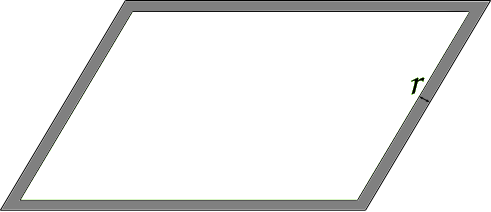
\includegraphics[scale=0.5]{tablefinie.png}
\caption{\label{tablefinie} The set $K(\mathbf{P},r)$ in grey}
\end{figure}

\begin{definition}
If $G$ is a unit distance graph, given with a unit distance representation 
$f:G\rightarrow \mathbb{R}^2$, let $\partial (G,f)$ be the diameter of the 
figure $f(G)$ in the plane.
\end{definition}

\begin{process}\label{toujours}
$G$ denotes a unit distance graph, and $r=\partial (G,f)$ for some 
unit legth representation $f$ of $G$.
\begin{itemize}
  \item let $\theta '$ (the orientation of our graph) be chosen uniformly 
  in $[0; 2 \pi[$ ;
  \item let $A_0$ be an independent point chosen uniformly in 
  $\mathbf{P} \setminus K(\mathbf{P},r)$ ;
  \item let $i$ be an independent index chosen uniformly in $[|1;m|]$.
\end{itemize}
Then, rotate the figure $f(G)$ by the angle $\theta$, translate it so that the origin 
falls on  $A_0$, and take the needle $(A',B')$ corresponding to the $i^{th}$ 
edge of the obtained graph. It is clearly inside of $\mathbf{P}$, by definition 
of $\partial(G,f)$.
\end{process}

\begin{lemma}
Denote by $p$ the probability that both ends have the same colour when throwing 
the needle with Process~\ref{encore}, an $p'$ for Process~\ref{toujours}, then 
$$ | p - p'| \leq \frac{\mathcal{A}(K(\mathbf{P},r))}{\mathcal{A}(\mathbf{P})} $$
where $r$ is still $\partial(G,f)$ for a representation $f$ of $G$.
\end{lemma}

\begin{proof}

\begin{eqnarray*}
|p' - p| 
  &=& | \mathbb{P}(A'_1 , A'_2 \in U_0) - \mathbb{P}(A_1 , A_2 \in U_0) + \mathbb{P}(A'_1 , A'_2 \in U_1) - \mathbb{P}(A_1 , A_2 \in U_1) | \\
  &\leq& | \mathbb{P}(A'_1 , A'_2 \in U_0) - \mathbb{P}(A_1 , A_2 \in U_0) | + | \mathbb{P}(A'_1 , A'_2 \in U_1) - \mathbb{P}(A_1 , A_2 \in U_1) | 
\end{eqnarray*}

Let's focus on the first term. 
Decompose the first probability in three terms corresponding to the final 
choice of $(A',B')$, $(A',C')$ or $(B',C')$, and the second one in three terms 
according to the position of $\theta$ :
\begin{eqnarray*}
& & \left| \mathbb{P}(A'_1 , A'_2 \in U_0) - \mathbb{P}(A_1 , A_2 \in U_0) \right| \\
&\leq& \frac{1}{3} \left| \mathbb{P}(A' \in U_0 , B' \in U_0) - \mathbb{P}(A_1 \in U_0 , A_1 + e^{i \theta} \in U_0 \ |\  \theta < \frac{\pi}{3} ) \right| \\
&+& \frac{1}{3} \left| \mathbb{P}(A' \in U_0 , C' \in U_0) - \mathbb{P}(A_1 \in U_0 , A_1 + e^{i \theta} \in U_0 \ |\  \frac{\pi}{3} \leq \theta < \frac{2 \pi}{3} ) \right| \\
&+& \frac{1}{3} \left| \mathbb{P}(B' \in U_0 ,C' \in U_0) - \mathbb{P}(A_1 \in U_0 , A_1 + e^{i \theta} \in U_0 \ | \  \frac{2 \pi}{3} > \theta ) \right|
\end{eqnarray*}

Once again, let's focus on the first term. When the points $A$ and 
$A'$ fall in $K(\mathbf{P},1)$, then the two points are uniformly distributed in 
$K(\mathbf{P},1)$, and independent of $\theta$ and $\theta'$. Thus we have : 
$$ \left| \mathbb{P}(A'_1 , A'_2 \in U_0) - \mathbb{P}(A_1 , A_2 \in U_0) \right| \leq \mathbb P(A \not \in K(\mathbf{P},1)) \leq \frac{\mathcal{A}(K(\mathbf{P},1))}{\mathcal{A}(\mathbf{P})} $$
\end{proof}
The proof can be adapted to circular tables, or more generally to any table 
whose shape is not too complicated.

We can similarly deduce bounds on the probabilities given by Process~\ref{encore}, 
since the ones given by Process~\ref{toujours} are always greater than $c_n(G)$.
For instance, taking an equilateral triangle with $2$ colours, we see that 
$p(c) \geq \frac13 - \frac{\mathcal{A}(K(\mathbf{P},1))}{\mathcal{A}(\mathbf{P})}$, 
if $p(c)$ is the probability given in Process~\ref{encore} by the $2$-colouring 
$c$ of $\mathbf{P}$. 
This bound becames sharp as parallelogram $\mathbf{P}$ becomes bigger.

\section{Final notes}
In the infinite case, it may seem a bit disappointing that we chose to study 
only periodic colourings. One can indeed hope for some similar results for a 
larger class of colourings. For instance, one can think of the probability $p_R$ 
of obtaining two same coloured endpoints when launching the needle on the ball 
$B(0,R)$ : we could have said that a colouring is \emph{valid} if $p_R$ converges 
as $R \rightarrow \infty$. If we denote $p$ this limit, section~\ref{fini} 
easily shows that we get the same main results for $p$, especially
Corollary~\ref{ineg} when taking $C_n$ the set of ``new'' valid colourings 
with $n$ colours. It's also clear that any periodic colouring is valid to that 
definition. Still, we chose not to use that notion, because $p$ is not a 
probability but what we may call an asymptotic probability, so it shouldn't be 
seen as a probability. It may though be the most natural way to give a sense to 
the (impossible) idea of ``throwing a needle uniformly on the whole plane''.
points $A$ and $A'$ fall on $\mathcal{P'}$, the two points are uniformly distributed in $\mathcal{P'}$, and independent of $\theta$ and $\theta'$. Thus this term is overestimated by the probability for $A$ and $A'$ to fall near the borders of the parallelogram. This probability is smaller than : $\mathcal{P}/\mathcal{A}$.

\end{document}
